\documentclass[tikz,border=10pt]{standalone}
\usepackage{tikz}

\begin{document}
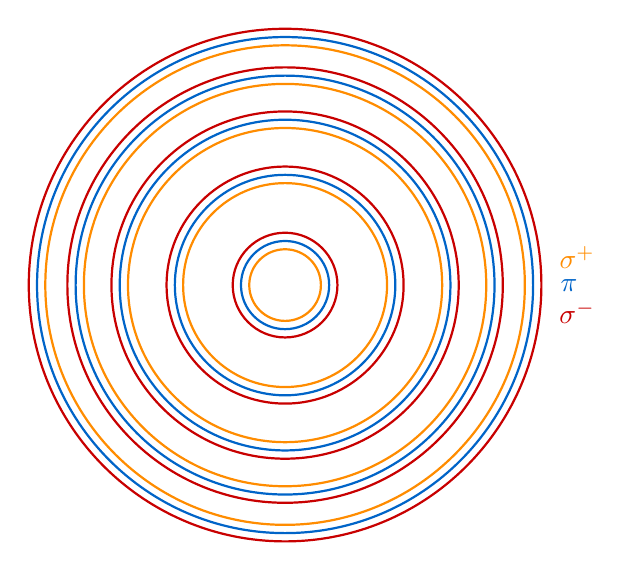
\begin{tikzpicture}[scale=0.7]

  \definecolor{sigmaplus}{RGB}{255, 140, 0}
  \definecolor{sigmaminus}{RGB}{200, 0, 0}
  \definecolor{unsplit}{RGB}{0, 100, 200}

  % Main rings (blue)
  \draw[thick, unsplit] (0, 0) circle (4.5);
  \draw[thick, unsplit] (0, 0) circle (3.8);
  \draw[thick, unsplit] (0, 0) circle (3.0);
  \draw[thick, unsplit] (0, 0) circle (2.0);
  \draw[thick, unsplit] (0, 0) circle (0.8);

  % Sigma^- rings (red, slightly larger = outer)
  \draw[thick, sigmaminus] (0, 0) circle (4.65);
  \draw[thick, sigmaminus] (0, 0) circle (3.95);
  \draw[thick, sigmaminus] (0, 0) circle (3.15);
  \draw[thick, sigmaminus] (0, 0) circle (2.15);
  \draw[thick, sigmaminus] (0, 0) circle (0.95);

  % Sigma^+ rings (orange, slightly smaller = inner)
  \draw[thick, sigmaplus] (0, 0) circle (4.35);
  \draw[thick, sigmaplus] (0, 0) circle (3.65);
  \draw[thick, sigmaplus] (0, 0) circle (2.85);
  \draw[thick, sigmaplus] (0, 0) circle (1.85);
  \draw[thick, sigmaplus] (0, 0) circle (0.65);

  % Labels
  \node[unsplit] at (5.15, 0)   {$\pi$};
  \node[sigmaminus] at (5.3, -0.5) {$\sigma^-$};
  \node[sigmaplus]  at (5.3,  0.5) {$\sigma^+$};

\end{tikzpicture}
\end{document}
